\documentclass{beamer}
% Use DS9 global theme (includes pgfplots for visualization)
\usepackage{../../../shared/templates/ds9_theme}

% Title page configuration
\title[If Else-If Else]{CS12 CH: If - Else If - Else}
\subtitle{Chaining Conditional Statements}
\author[Mr. Gullo]{Mr. Gullo}
\date[Oct 2024]{October 2024}

\begin{document}
\frame{\titlepage}

\section{Introduction}

\begin{frame}
\frametitle{Learning Objectives}
By the end of this lesson, you will be able to:
\begin{itemize}
    \item Understand the structure and flow of \texttt{if-else if-else} statements\pause
    \item Identify when to use \texttt{else if} for mutually exclusive conditions\pause
    \item Recognize and eliminate redundant conditions in conditional chains\pause
    \item Apply \texttt{if-else if-else} statements to solve classification problems\pause
    \item Debug common logic errors in multi-branch conditionals
\end{itemize}
\end{frame}

\section{Instructor Notes}

\begin{frame}
\frametitle{Demo Programs for This Lesson}
\textbf{Programs to demonstrate live:}
\begin{itemize}
    \item \texttt{1elseif\_skeleton.cpp} - Basic structure of else if chain (divisibility by 2 and 3)
    \item \texttt{2elseif\_posNeg.cpp} - Classifying numbers as positive, negative, or zero
    \item \texttt{3elseif\_2\_3.cpp} - Same as skeleton (divisibility testing)
    \item \texttt{4elseif\_bad.cpp} - Age classification with redundant conditions (teaching moment)
\end{itemize}

\vspace{0.3cm}
\textbf{Location:} \texttt{lessonPrograms/}

\vspace{0.3cm}
\alert{Note:} These are for instructor demonstration only. Use to show proper else-if structure and common pitfalls.
\end{frame}

\section{Conditional Chaining Concepts}

\begin{frame}
\frametitle{Why Else If?}
\textbf{Problem:} Sometimes we need to check multiple mutually exclusive conditions.\pause

\vspace{0.3cm}
\textbf{Example Scenario:}
\begin{itemize}
    \item Is a number positive, negative, or zero?
    \item What age category does a person fall into?
    \item Which commission bracket applies to a sales amount?
\end{itemize}\pause

\vspace{0.3cm}
\textbf{Key Insight:} Only ONE of these conditions should execute, and we should stop checking once we find a match.
\end{frame}

\begin{frame}
\frametitle{The If - Else If - Else Structure}

\begin{center}
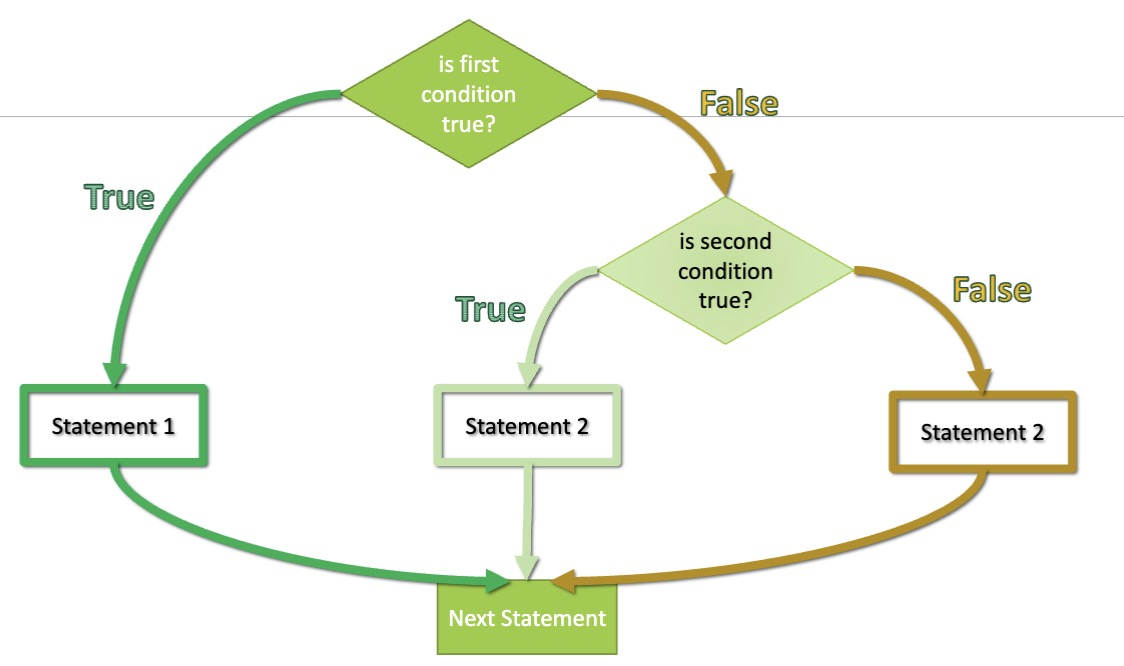
\includegraphics[width=0.8\textwidth]{../images/06_else-if-flowchart.jpg}
\end{center}
\end{frame}

\begin{frame}[fragile]
\frametitle{Syntax Structure}
\textbf{General Form:}
\begin{minted}[fontsize=\small, frame=lines]{cpp}
if (condition1) {
    // Statement 1
}
else if (condition2) {
    // Statement 2
}
else if (condition3) {
    // Statement 3
}
else {
    // Default statement
}
// Next statement (continues here)
\end{minted}

\textbf{Important:} Only ONE block executes, then control moves to next statement.
\end{frame}

\section{Simple Examples}

\begin{frame}[fragile]
\frametitle{Example 1: Positive, Negative, or Zero}
\textbf{Demo File:} \texttt{2elseif\_posNeg.cpp}

\begin{minted}[fontsize=\small, frame=lines, linenos]{cpp}
#include <iostream>
using namespace std;

int main() {
    int testNumber;
    
    cout << "Please enter an integer: ";
    cin >> testNumber;
    
    if(testNumber < 0)
        cout << testNumber << " is negative.\n";
    else if(testNumber > 0)
        cout << testNumber << " is positive\n";
    else
        cout << testNumber << " is zero.";
    
    return 0;
}
\end{minted}
\end{frame}

\begin{frame}[fragile]
\frametitle{Example 2: Divisibility Testing}
\textbf{Demo File:} \texttt{1elseif\_skeleton.cpp}

\begin{minted}[fontsize=\scriptsize, frame=lines, linenos]{cpp}
#include <iostream>
using namespace std;

int main() {
    int testNumber;
    
    cout << "Please enter an integer: ";
    cin >> testNumber;
    
    if(testNumber % 6 == 0)
        cout << testNumber << " is divisible by 2 and 3\n";
    else if(testNumber % 2 == 0)
        cout << testNumber << " is divisible by 2 but not 3\n";
    else if(testNumber % 3 == 0)
        cout << testNumber << " is divisible by 3 but not 2\n";
    else
        cout << testNumber << " is neither divisible by 3 nor 2\n";
    
    return 0;
}
\end{minted}
\end{frame}

\begin{frame}
\frametitle{Why Check Divisibility by 6 First?}
\textbf{Consider:} What happens if we enter the number 12?\pause

\begin{itemize}
    \item 12 is divisible by 2 \checkmark
    \item 12 is divisible by 3 \checkmark
    \item 12 is divisible by 6 \checkmark
\end{itemize}\pause

\vspace{0.3cm}
\textbf{Order Matters!}
\begin{itemize}
    \item If we check \texttt{testNumber \% 2 == 0} first, we'd say "divisible by 2 but not 3"
    \item This would be WRONG for 6, 12, 18, etc.
    \item Must check the MOST SPECIFIC condition first
\end{itemize}
\end{frame}

\section{Redundant Conditions}

\begin{frame}[fragile]
\frametitle{Common Mistake: Redundant Conditions}
\textbf{Demo File:} \texttt{4elseif\_bad.cpp} (Why is this called "bad"?)\pause

\begin{minted}[fontsize=\scriptsize, frame=lines, linenos]{cpp}
if(userAge <= 1)
    cout << "The user is an infant\n";
else if(userAge >= 2 && userAge <= 12)
    cout << "The user is a child\n";
else if(userAge >= 13 && userAge <= 19)
    cout << "The user is an teenager\n";
else
    cout << "The user is an adult\n";
\end{minted}

\vspace{0.3cm}\pause
\textbf{Question:} Is \texttt{userAge >= 2} necessary on line 3?
\end{frame}

\begin{frame}
\frametitle{Understanding Redundant Conditions}
\textbf{Analysis:}
\begin{itemize}
    \item First condition: \texttt{userAge <= 1}\pause
    \item If this is FALSE, what do we know?\pause
    \item We know: \texttt{userAge > 1}, which means \texttt{userAge >= 2}\pause
    \item So checking \texttt{userAge >= 2} is REDUNDANT
\end{itemize}\pause

\vspace{0.3cm}
\textbf{Key Principle:} When an \texttt{else if} executes, ALL previous conditions are already known to be false. Use this information to simplify your conditions!
\end{frame}

\begin{frame}[fragile]
\frametitle{Improved Version}
\textbf{Better Code (No Redundancy):}

\begin{minted}[fontsize=\small, frame=lines, linenos]{cpp}
if(userAge <= 1)
    cout << "The user is an infant\n";
else if(userAge <= 12)
    cout << "The user is a child\n";
else if(userAge <= 19)
    cout << "The user is an teenager\n";
else
    cout << "The user is an adult\n";
\end{minted}

\vspace{0.3cm}\pause
\textbf{Why this works:}
\begin{itemize}
    \item Line 3: We know \texttt{userAge > 1}, so just check upper bound
    \item Line 5: We know \texttt{userAge > 12}, so just check upper bound
    \item Line 7: We know \texttt{userAge > 19}, so must be adult
\end{itemize}
\end{frame}

\section{Practice Exercises}

\begin{frame}[fragile]
\frametitle{Exercise 1: Sales Commission Calculator}
\textbf{Problem:} Calculate commission based on total sales.

\vspace{0.2cm}
\begin{tabular}{|l|l|}
\hline
\textbf{Sales Amount} & \textbf{Commission Rate} \\
\hline
\$0 - \$10,000 & 5\% \\
\$10,001 - \$50,000 & 8\% \\
\$50,001 - \$100,000 & 10\% \\
Over \$100,000 & 12\% \\
\hline
\end{tabular}

\vspace{0.3cm}
\textbf{Task:} Write a program that:
\begin{itemize}
    \item Prompts user for total sales
    \item Calculates income (commission)
    \item Outputs the result
\end{itemize}
\end{frame}

\begin{frame}[fragile]
\frametitle{Exercise 1: Template with TODOs}

\begin{minted}[fontsize=\scriptsize, frame=lines, linenos, breaklines]{cpp}
#include <iostream>
using namespace std;

int main() {
    double sales, commission;
    
    cout << "Enter total sales: $";
    cin >> sales;
    
    // TODO 1: Check if sales <= 10000, calculate 5% commission
    
    // TODO 2: Check if sales <= 50000, calculate 8% commission
    
    // TODO 3: Check if sales <= 100000, calculate 10% commission
    
    // TODO 4: For sales > 100000, calculate 12% commission
    
    // TODO 5: Output the commission with appropriate formatting
    
    return 0;
}
\end{minted}
\end{frame}

\begin{frame}[fragile]
\frametitle{Exercise 2: Coordinate Classification}
\textbf{Problem:} Given a point $(x, y)$, determine its location:
\begin{itemize}
    \item At the origin , On the x-axis (not origin), On the y-axis (not origin), In quadrant 1, 2, 3, or 4
\end{itemize}

\begin{center}
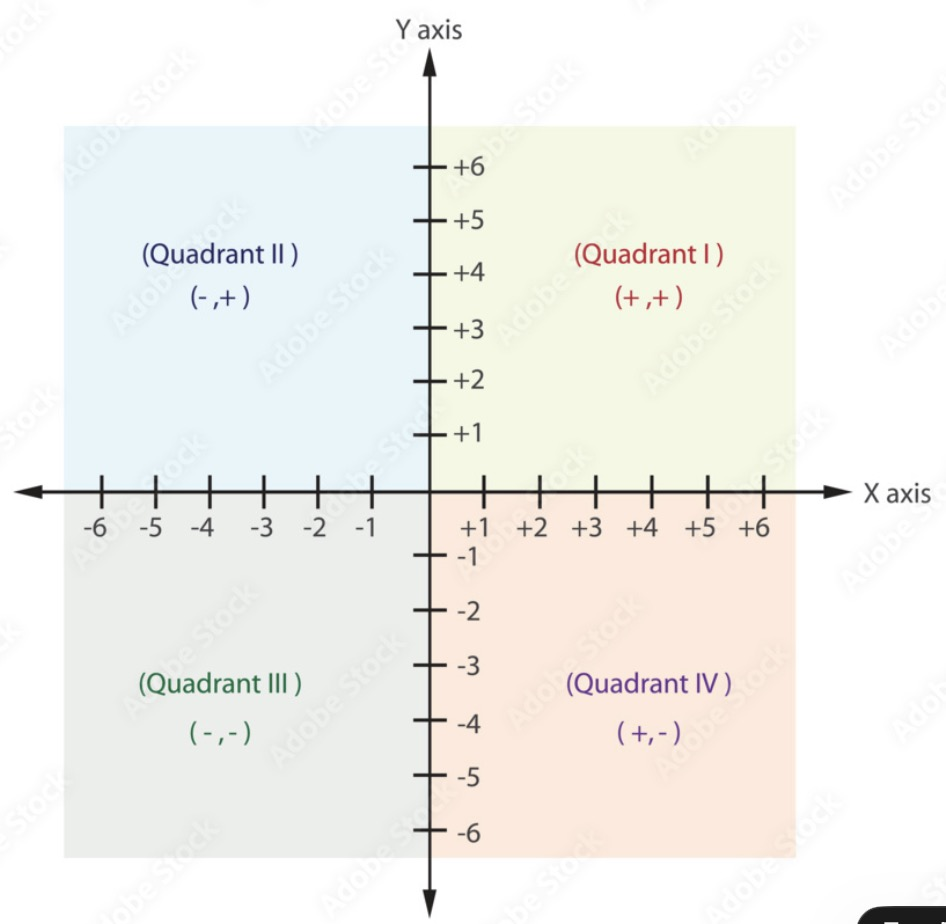
\includegraphics[width=0.5\textwidth]{../images/06_coordinate-plane-quadrants.jpg}
\end{center}

\vspace{0.2cm}
\textbf{Hints:}
\begin{itemize}
    \item Origin: both $x = 0$ and $y = 0$
    \item X-axis: $y = 0$ (but not origin)
    \item Y-axis: $x = 0$ (but not origin)
    \item Quadrant 1: $x > 0$ and $y > 0$
\end{itemize}
\end{frame}

\begin{frame}[fragile]
\frametitle{Exercise 2: Template with TODOs}

\begin{minted}[fontsize=\scriptsize, frame=lines, linenos, breaklines]{cpp}
#include <iostream>
using namespace std;

int main() {
    double x, y;
    
    cout << "Enter x coordinate: ";
    cin >> x;
    cout << "Enter y coordinate: ";
    cin >> y;
    
    // TODO 1: Check if at origin (x==0 AND y==0)
    
    // TODO 2: Check if on x-axis (y==0, but not origin)
    
    // TODO 3: Check if on y-axis (x==0, but not origin)
    
    // TODO 4-7: Check for each quadrant
    
    return 0;
}
\end{minted}
\end{frame}

\section{Common Pitfalls}

\begin{frame}
\frametitle{Common Mistakes to Avoid}
\textbf{1. Wrong Order of Conditions}
\begin{itemize}
    \item Always check MORE SPECIFIC conditions first
    \item Example: Check "divisible by 6" before "divisible by 2"
\end{itemize}\pause

\vspace{0.3cm}
\textbf{2. Redundant Conditions}
\begin{itemize}
    \item Remember: \texttt{else if} means all previous conditions were false
    \item Use this knowledge to simplify your conditions
\end{itemize}\pause

\vspace{0.3cm}
\textbf{3. Forgetting the Final Else}
\begin{itemize}
    \item Final \texttt{else} catches all remaining cases
    \item Prevents unexpected behavior for edge cases
\end{itemize}
\end{frame}

\begin{frame}[fragile]
\frametitle{Debugging Strategy}
\textbf{When your else-if chain doesn't work:}

\begin{enumerate}
    \item Test each condition boundary
    \item Print which condition matched
    \item Check for overlapping conditions
    \item Verify order is from specific to general
\end{enumerate}\pause

\vspace{0.3cm}
\textbf{Example Debug Output:}
\begin{minted}[fontsize=\small]{cpp}
if(condition1) {
    cout << "Branch 1 executed\n";
    // rest of code
}
else if(condition2) {
    cout << "Branch 2 executed\n";
    // rest of code
}
\end{minted}
\end{frame}

\section{Student Assignment}

\begin{frame}
\frametitle{Homework Assignment}
\textbf{Complete the following exercises:}

\begin{enumerate}
    \item Sales Commission Calculator (Exercise 1)
    \item Coordinate Classification (Exercise 2)
    \item Grade Letter Assignment:
    \begin{itemize}
        \item A: 90-100
        \item B: 80-89
        \item C: 70-79
        \item D: 60-69
        \item F: Below 60
    \end{itemize}
\end{enumerate}

\vspace{0.3cm}
\textbf{Submission Format:}
\begin{itemize}
    \item \texttt{firstnameLastname\_elseif.cpp}
    \item Include all three exercises in separate functions
    \item Test with multiple inputs
    \item Submit via Schoology by due date
\end{itemize}
\end{frame}

\begin{frame}
\frametitle{Assessment Resources}
\textbf{Practice Quiz Available:}
\begin{itemize}
    \item 12 multiple-choice questions on if-else if-else
    \item Located in \texttt{Relational Expression THW} folder
    \item Focus areas:
    \begin{itemize}
        \item Understanding flow control
        \item Identifying redundant conditions
        \item Determining correct output
        \item Order of condition checking
    \end{itemize}
\end{itemize}

\vspace{0.3cm}
\alert{Reminder:} Practice makes perfect! Try writing your own classification problems.
\end{frame}

\section{Summary}

\begin{frame}
\frametitle{Key Takeaways}
\begin{itemize}
    \item \texttt{if-else if-else} chains handle mutually exclusive conditions\pause
    \item Only ONE branch executes, then control skips to next statement\pause
    \item Order matters: check MORE SPECIFIC conditions first\pause
    \item Eliminate redundant conditions using logical implications\pause
    \item Always include final \texttt{else} to catch remaining cases\pause
    \item Test boundary values and edge cases thoroughly
\end{itemize}

\vspace{0.5cm}
\textbf{Next Lesson:} Switch statements and loops for more complex control flow!
\end{frame}

\end{document}
